\chapter{Results}
\label{cha:result}
Experiments \fix{TODO}
In this chapter we present the results of the experiments performed on the end to end model in \ref{design}. The goal of this section is to  present the conditions under which this type of model performs well, and likewise to determine when it does not. 

\begin{itemize}
    \item Section \ref{toygauss}: This section covers the application of our model to a simple toy dataset, designed to test the hypothesised advantages over traditional methods.
    
 
\end{itemize} \pagebreak



\section{Toy Example: Gaussian data}
\label{toygauss}
The first situation where we will test our model is a synthetic dataset. We want this data constructed in such a way as to test the underlying hypothesis motivating the model in \ref{design}. That is, our end to end model can improve performance in cases where standard dimensionality reduction removes potentially useful information.

In order to appropriately test this, we therefore want our data to contain useful information which we expect standard methods to ignore. The approach we take to construct this is to take a $d$ dimensional Gaussian, with mutually independent components for simplicity. The covariance matrix is then composed of the diagonal variance entries of each dimension. The important point here is to set the variance of each dimension to be largely different in magnitude. Since the covariance between dimensions is zero, we would expect the coordinate system of dimensionality reduction methods to be focused on the axes with the largest variance. We expect this coordinate system to contain little information on the lower variance dimensions.  If the supervised learning target is a function of these lower dimensions, we would therefore expect to see low performance when using these as features. In contrast, the use of a combined model has the signal of supervised loss as a factor in the choice of representation. It should choose a representation which still preserves the important information in the lower variance features. So we expect to see an improvement in performance for this type of data when using our model in comparison to baseline methods. \\

Formally, we generate this data by taking $n$ draws from a $d$ dimensional Gaussian denoting the variance for each component (i.e. the diagonals of the covariance matrix) as $\sigma_1, ..., \sigma_d$. From above, we note that $\sigma_1 >>  ... >> \sigma_d$. Then we define our $n\times d$ data matrix $\mathbf{X}$, with each $\mathbf{x}_i \sim \mathcal{N}(\mathbf{0}, \Sigma)$. Since CoDA requires non-negative values, we scale each axis by the minimum value if it is negative. Our targets will then be a function of the least variant axis, $\mathbf{y} = f(\mathbf{x}_j), j = 1,...,d$ (where $j$ is indexing $\mathbf{X}$ by columns i.e. axes).  \\

Figure \ref{} shows an example of synthetic data constructed in such a way. We note the large difference in the spread of the data between the axes, and 


Implementing this, we 

From our results, we can clearly see the advantage of an end to end model over baselines when the targets are a function of the least variant axis. An interesting experiment to follow this is to invetigate how this performance differential changes as the targets become a function of more variant axes. 

add results 

discuss

\subsection{Hyperparameter Grid Search}
Below we present the results from the 3 trial hyperparameter grid search protocol we introduced in \ref{cha:methodology}.  





\section{CoDA-PCA Microbiome data}
Smallish for both dimensions, uses OTUs at genus level

Still no improvement over baseline using end to end. Even with larger sample size (1000), performance is at best the same, often much lower.  

\section{RUG}
New microbiome results, using species level  
- Poor performance, can't do better than chance
- Why?: Sheer depth of connections needed in 'fat' matrices to map them to a lower dimension. The small sample size does not allow for enough information for the network to establish meaningful relationships between the input, low level representation and the output. 
- Preprocessing with dim reduction works better because the dimensionality reduction algorithms are fixed, and there is no need to learn them unlike in the network.
- Can see from 2D/3D plots there is not enough information in these dimensions to meaningfully distinguish classes. Also note the different representations of PCA and CoDA-PCA

A lot of modern results are of this 'fat' form, given the small sample sizes and large diversity in microbiome species. To improve performance/reduce size it may make sense to do analysis at the genus or higher level. 

https://microbiomedb.org/mbio/app/ other sources if needed

%\section{Direct Cost}\
%\label{sec:direct_cost}

%Here is the example to show how to include a figure. %Figure~\ref{fig:cost}
%includes two subfigures (Figure~\ref{fig:zerocost}, and %Figure~\ref{fig:zerobus});

%\begin{figure*}
%  \label{fig:cost}
%  \subfigure[Fraction of cycles spent on %zeroing\label{fig:zerocost}]{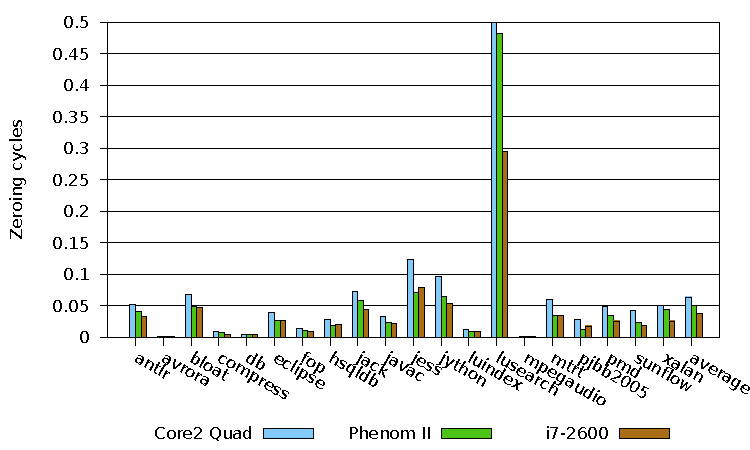
\includegraphics[width=\columnwidth]{f%igs/zerocost_intel.pdf}}
%  \subfigure[BytesZeroed / %BytesBurstTransactionsTransferred\label{fig:zerobus}]{\includegraph%ics[width=1.0\columnwidth]{figs/zerobus_core.pdf}}
%  \caption{The cost of zero initialization}
%\end{figure*}


\section{Summary}
